\section{Motor Assembly}
\label{sec:motor-assembly}
\resetassemblysteps

%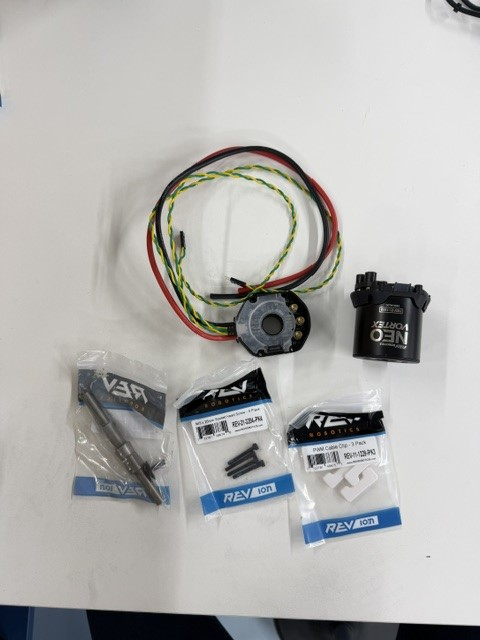
\includegraphics[width=2in,height=1.94723in]{media/image1.jpg}

\begin{partsbox}
\begin{tabularx}{\linewidth}{@{}X m{0.28\linewidth}@{}}
\begin{minipage}[t]{\linewidth}
\vspace{0pt}
\begin{itemize}
    \item 8 \href{https://www.revrobotics.com/rev-21-1652/}{NEO Vortex Brushless Motors}
    \item 8 \href{https://www.revrobotics.com/rev-11-2159/}{SPARK Flex Motor Controllers}
    \item 8 \href{https://www.revrobotics.com/rev-21-2807/}{Vortex Shafts -- 8mm}
\end{itemize}
\end{minipage}
&
\begin{minipage}[t]{\linewidth}
\vspace{0pt}
\centering
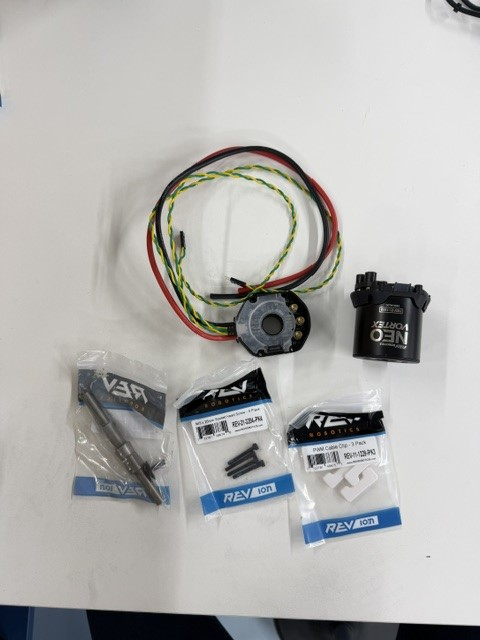
\includegraphics[
    width=\linewidth,
    trim=1.2cm 1.2cm 1.2cm 3.5cm,
    clip
]{media/image1.jpg}
\end{minipage}
\end{tabularx}
\end{partsbox}

This section describes how to assemble the NEO Vortex motor with the SPARK Flex motor controller and install the output shaft prior to mounting the assembly to the swerve module.
\clearpage
\assemblystep{Install the Motor Controller}
Align the three circular pins and the rectangular connector on the motor
and controller and firmly press together.

\begin{figure}[H]
\centering
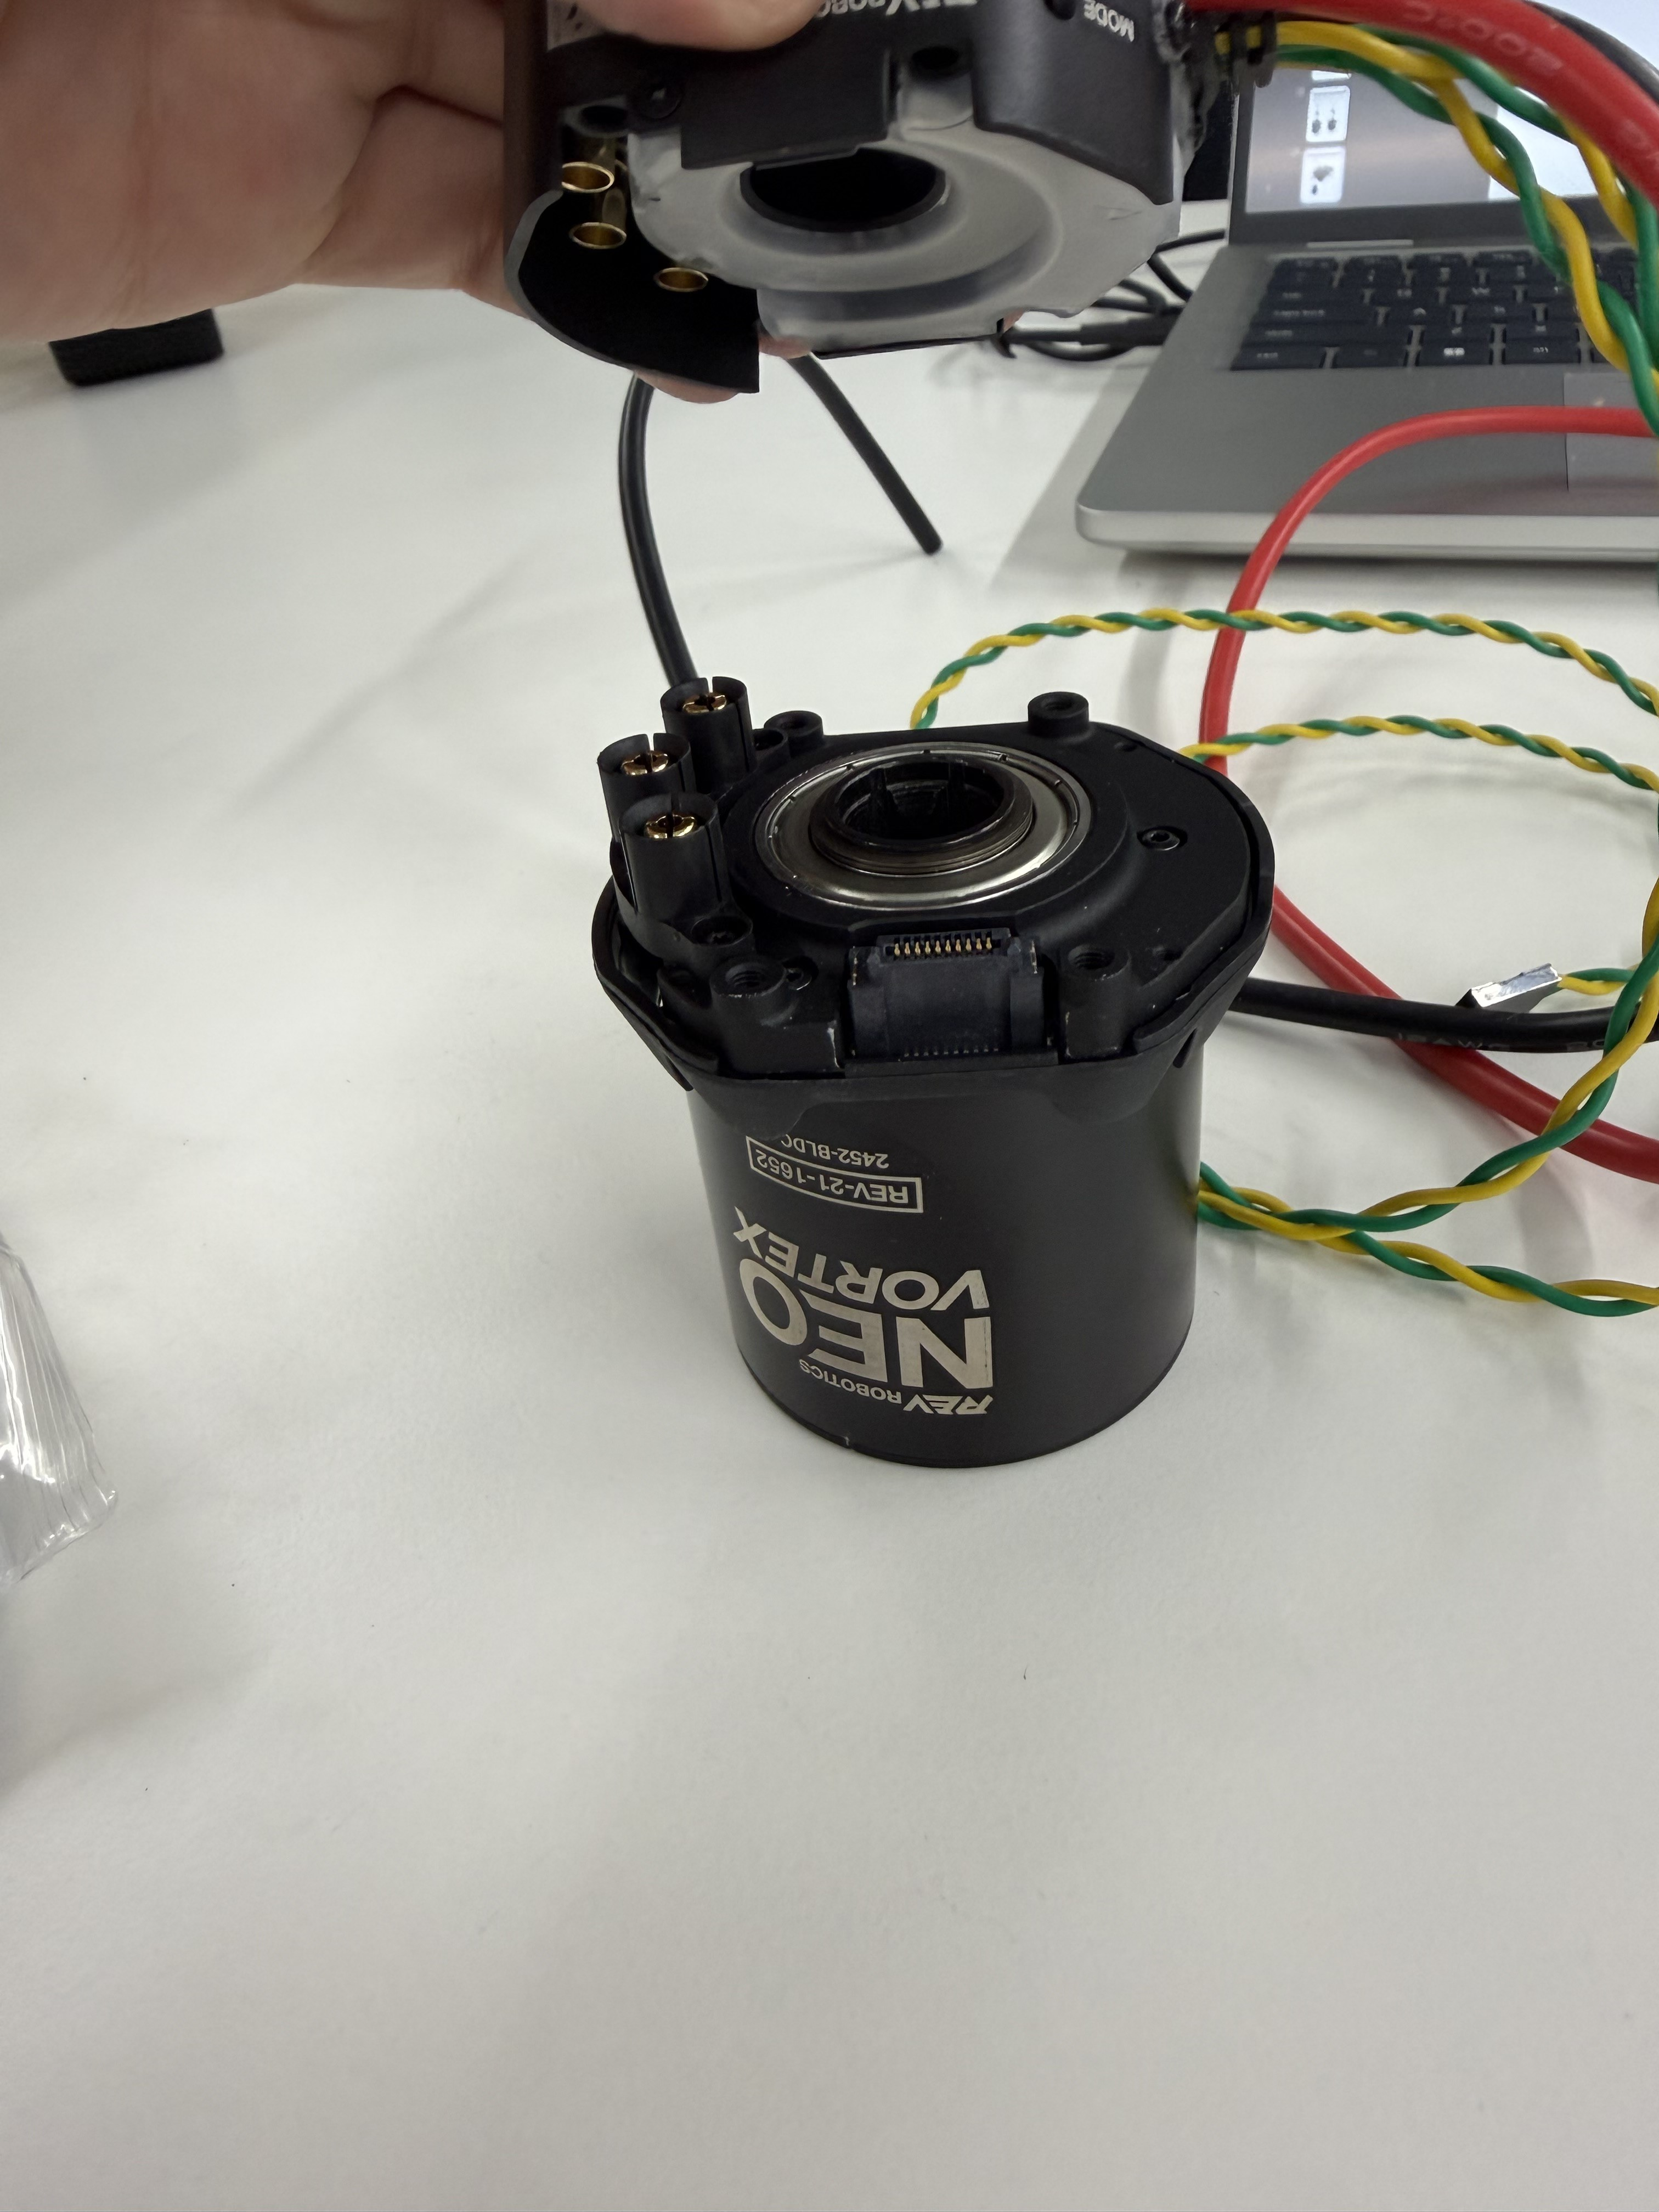
\includegraphics[width=0.47\textwidth]{media/image2.jpg}
\hfill
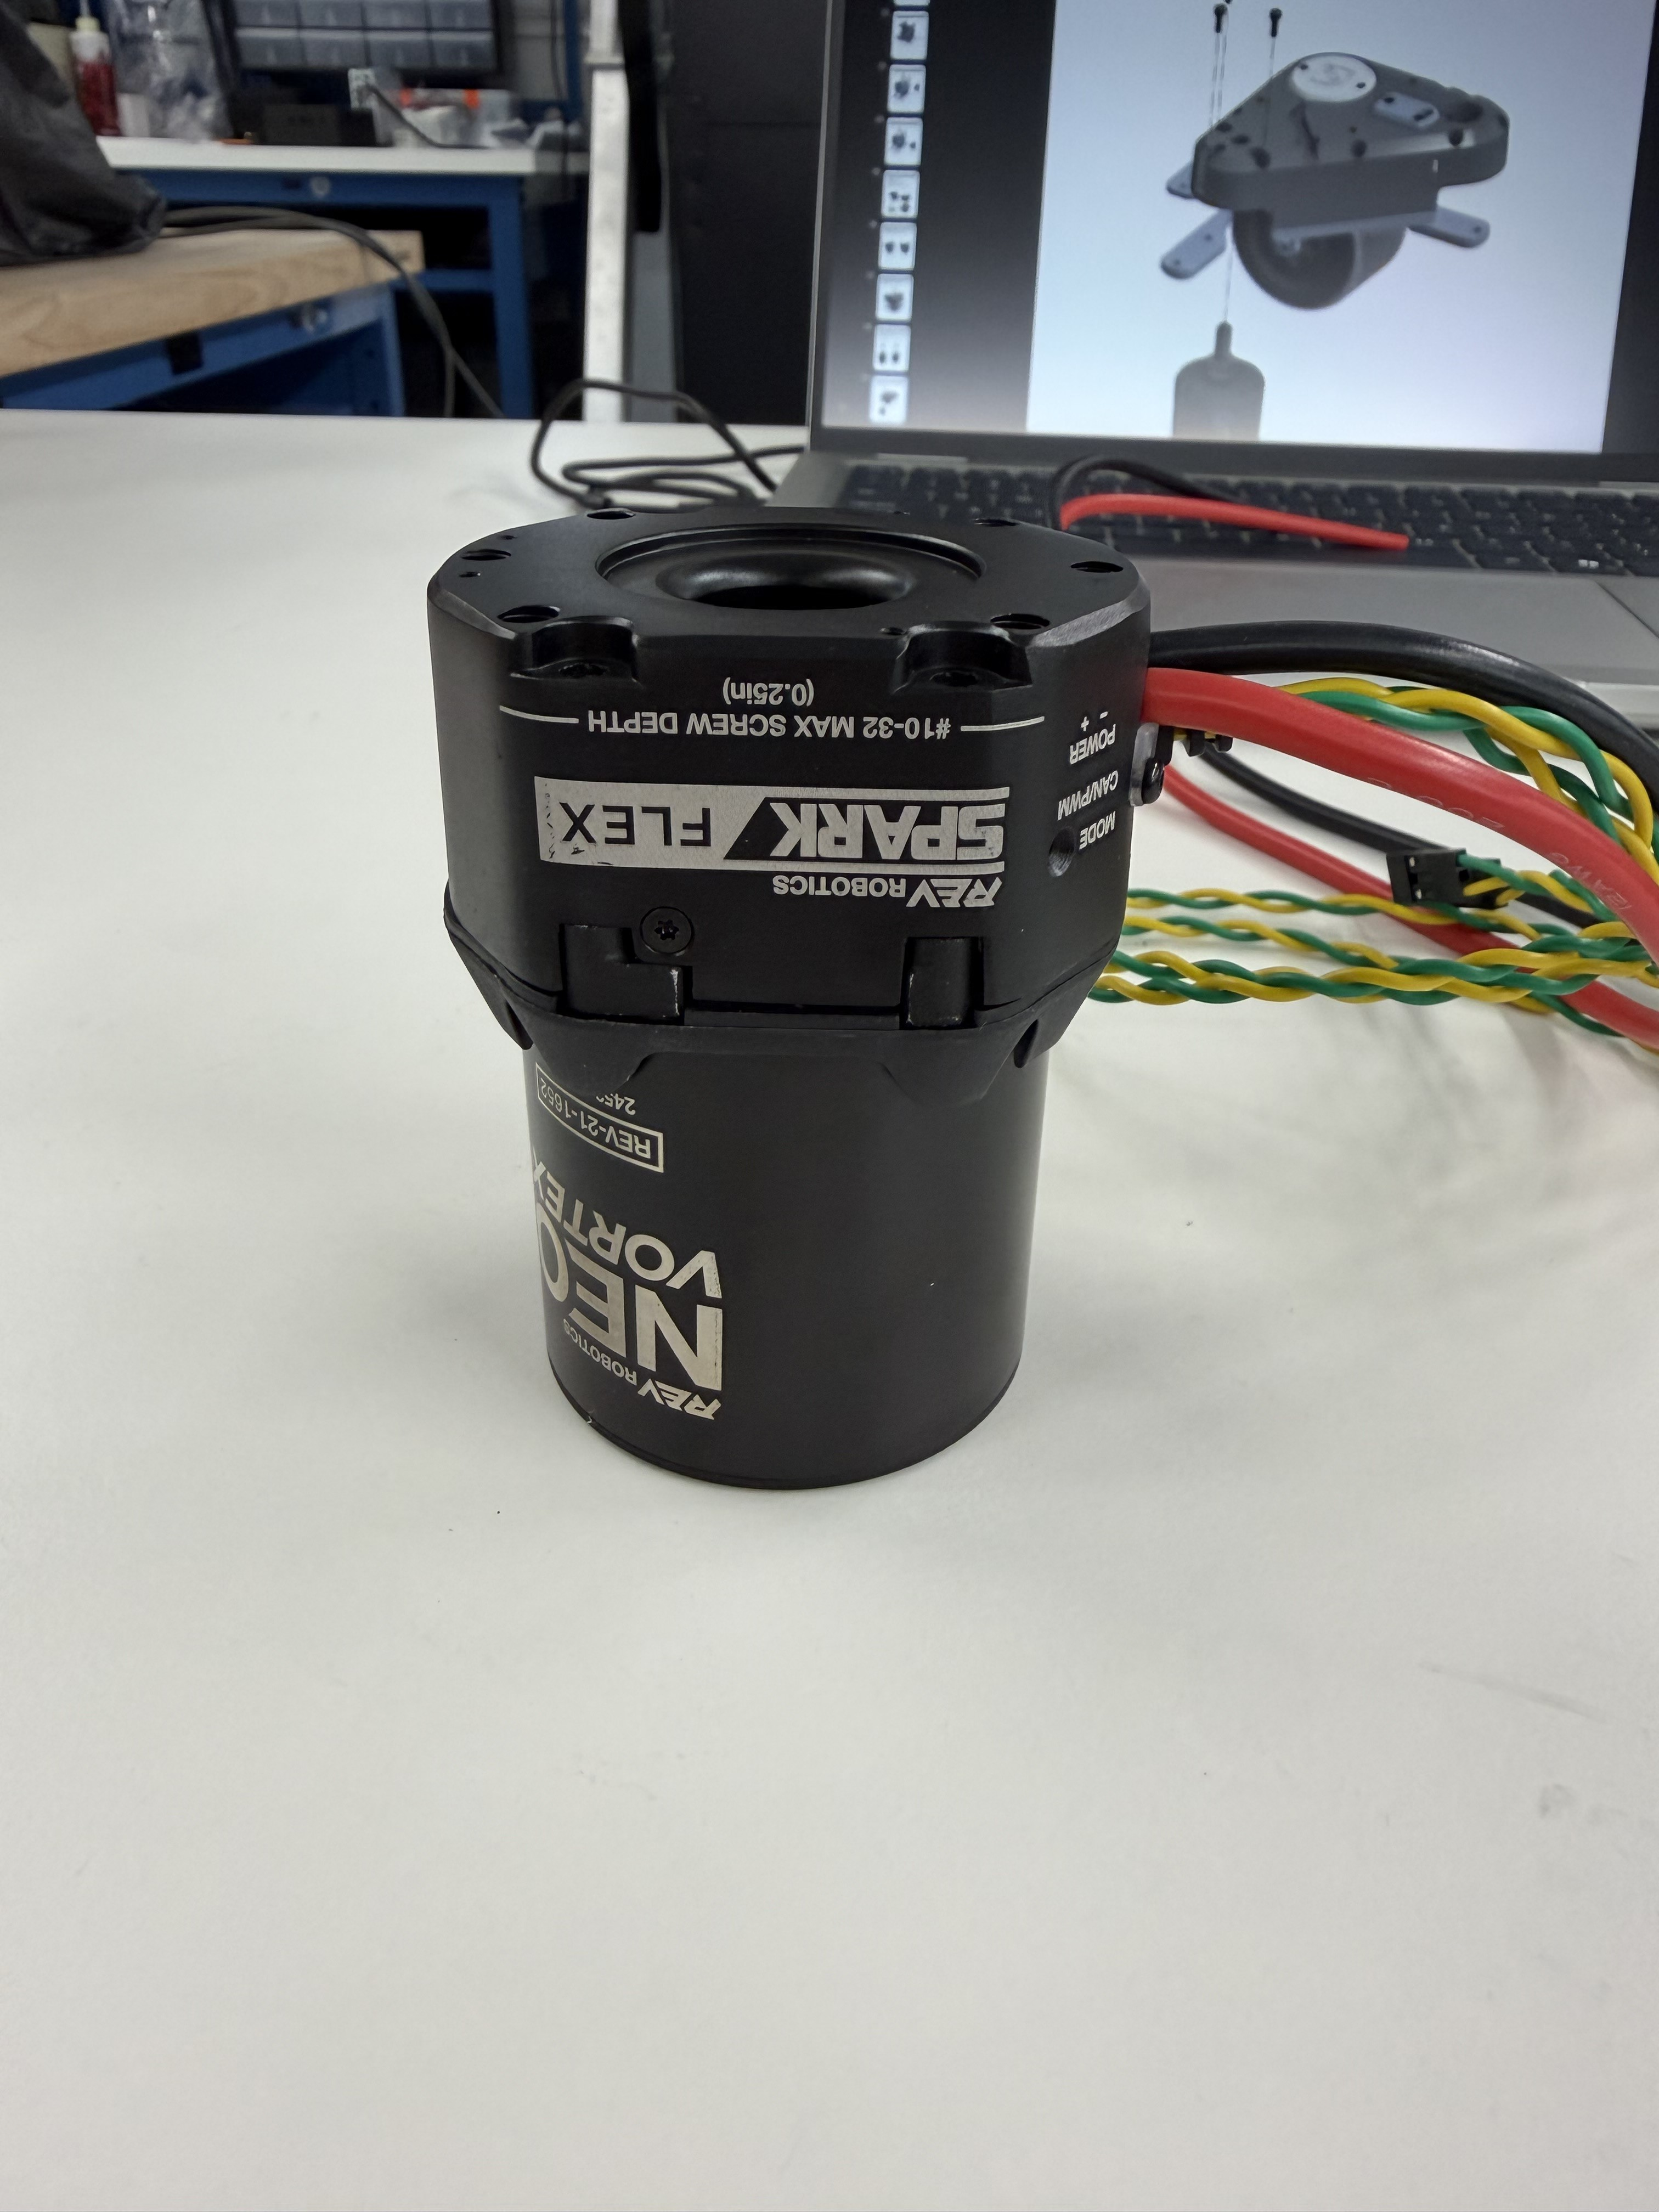
\includegraphics[width=0.47\textwidth]{media/image3.jpg}
\caption{Aligning the pins and connector, then pressing the controller
onto the motor body.}
\end{figure}

\assemblystep{Secure the Controller}
Insert the 4 provided screws into the inset holes on top of the controller (text pointing downwards) to firmly attach the
controller.
\begin{warningbox}
Do not overtighten the controller screws.
\end{warningbox}
%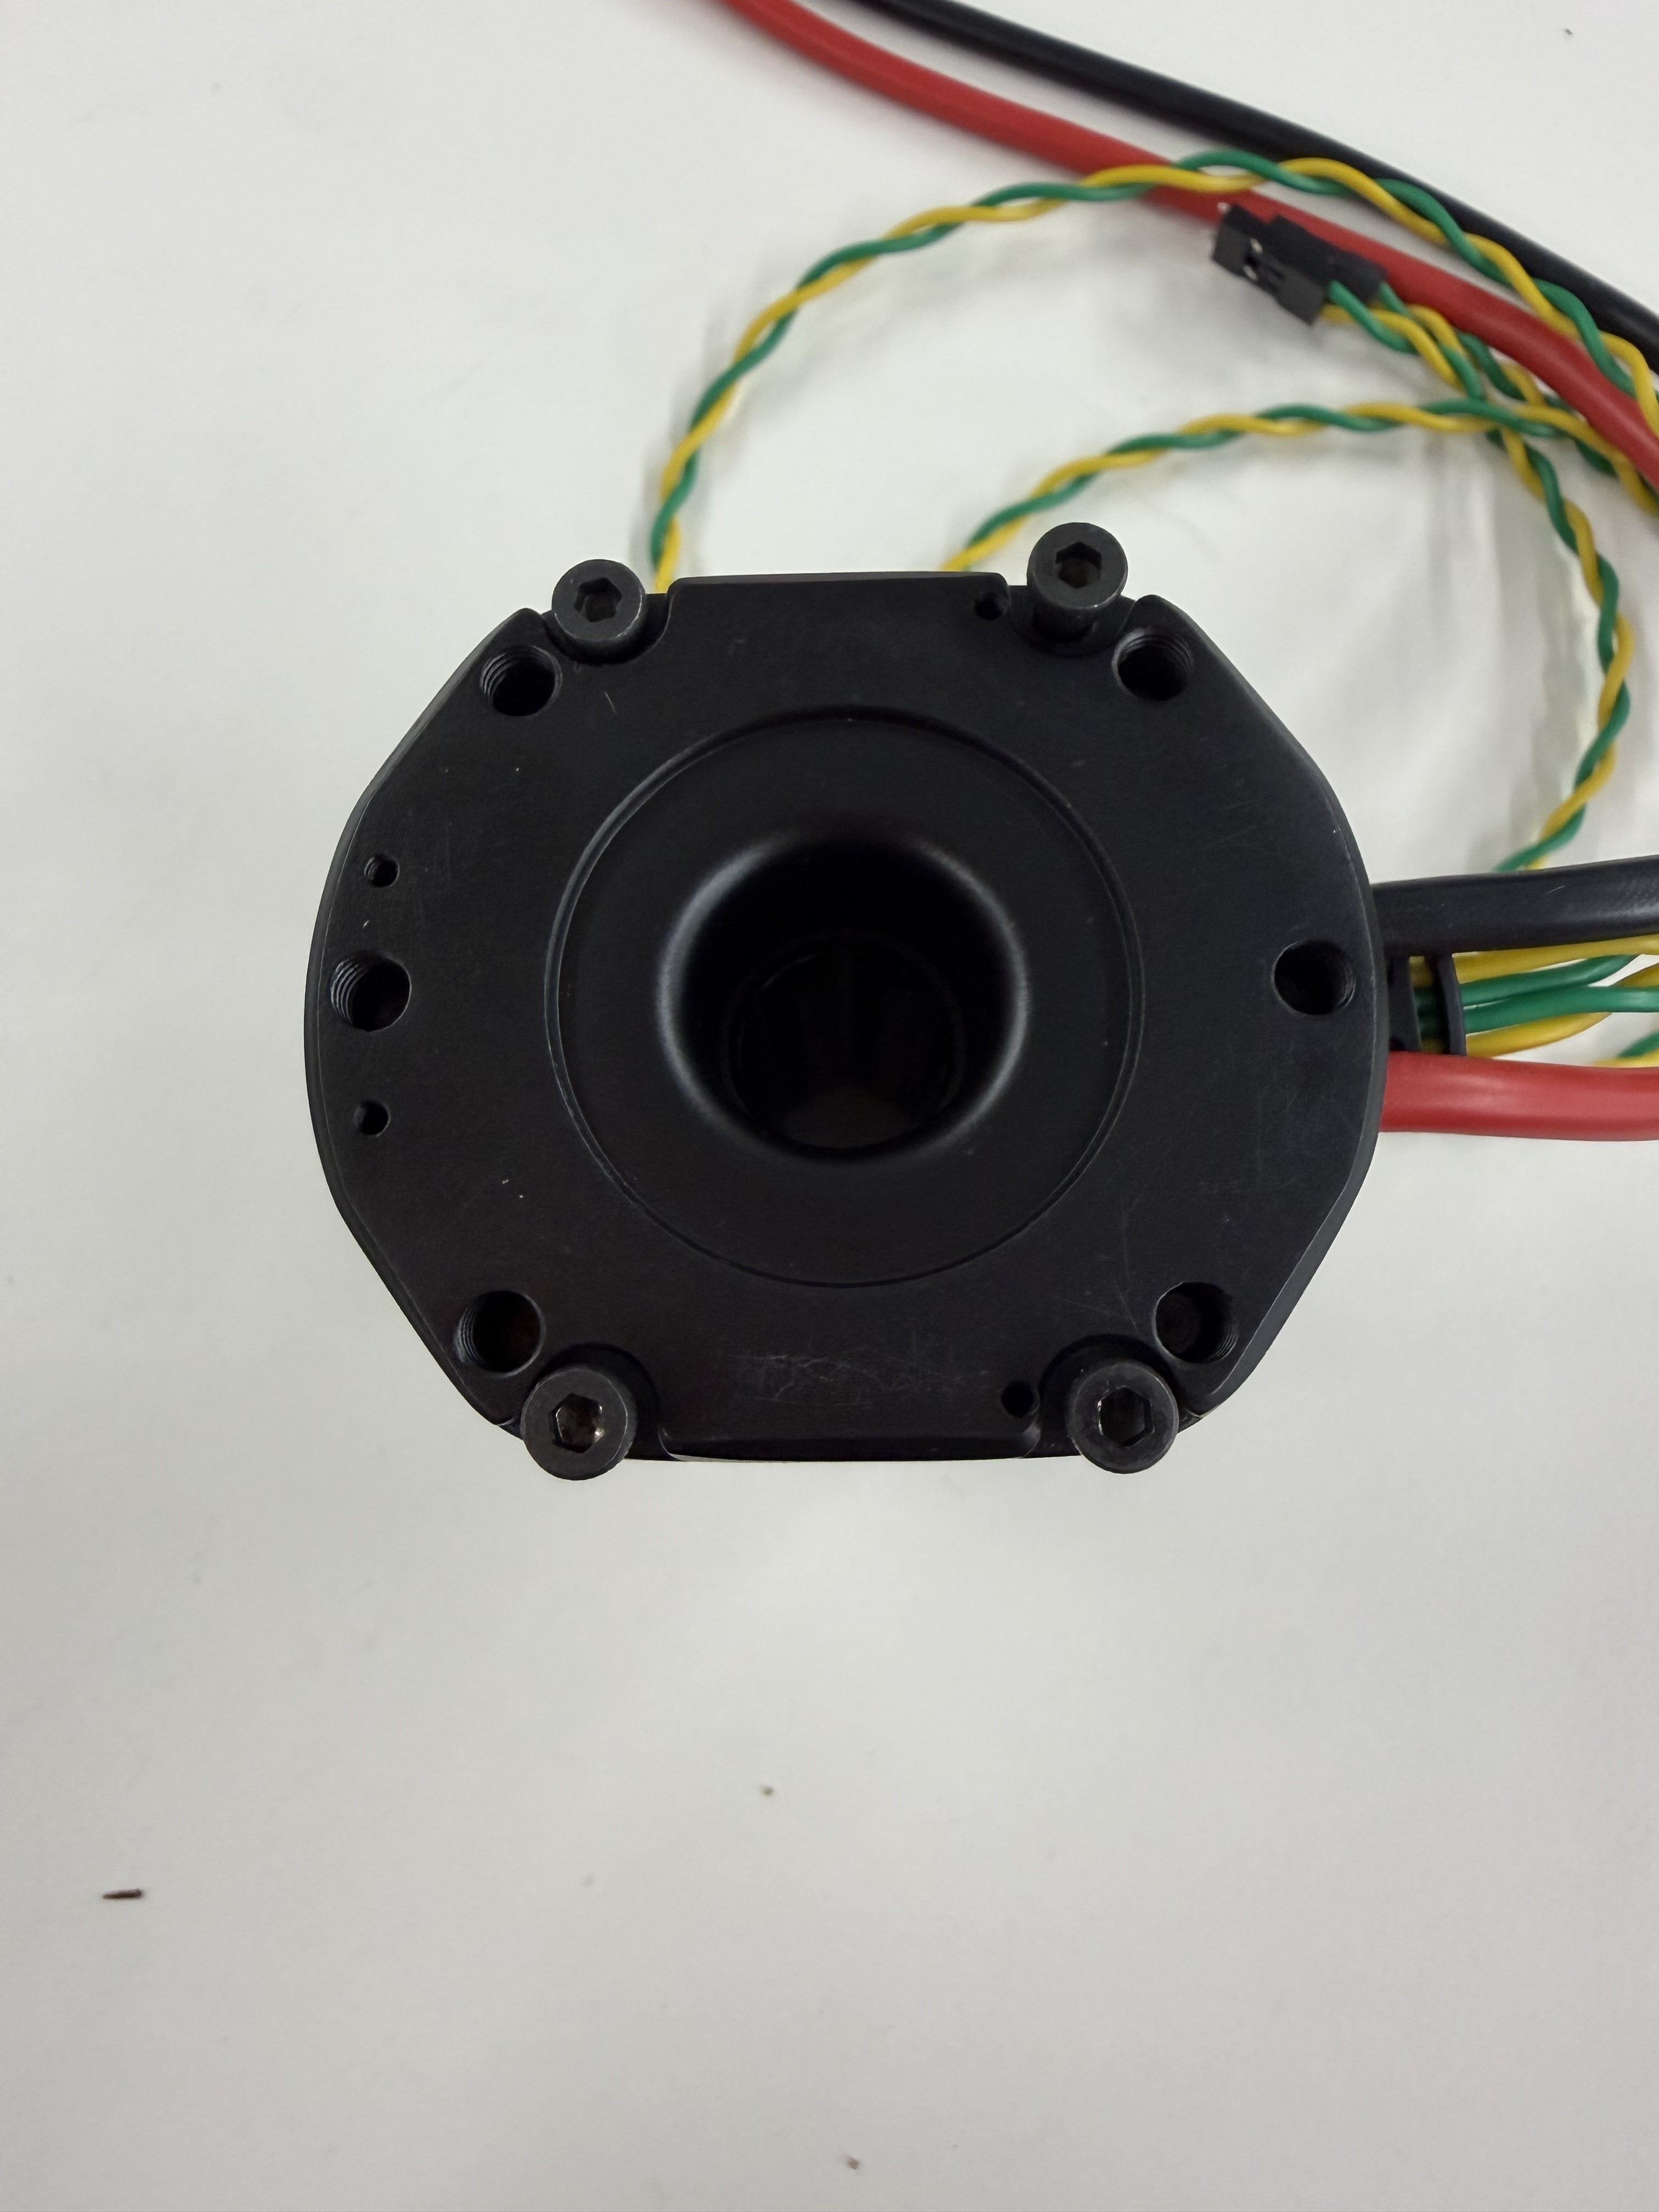
\includegraphics[width=2in,height=1.93557in]{media/image4.jpg}
\clearpage
\assemblystep{Install the Shaft}
With the controller on top, insert the motor shaft into the center of
the motor. The side with the groove along the shaft should be facing
upwards. Then use the provided screw to secure the shaft from the
opposite side of the motor.

\begin{figure}[H]
\centering
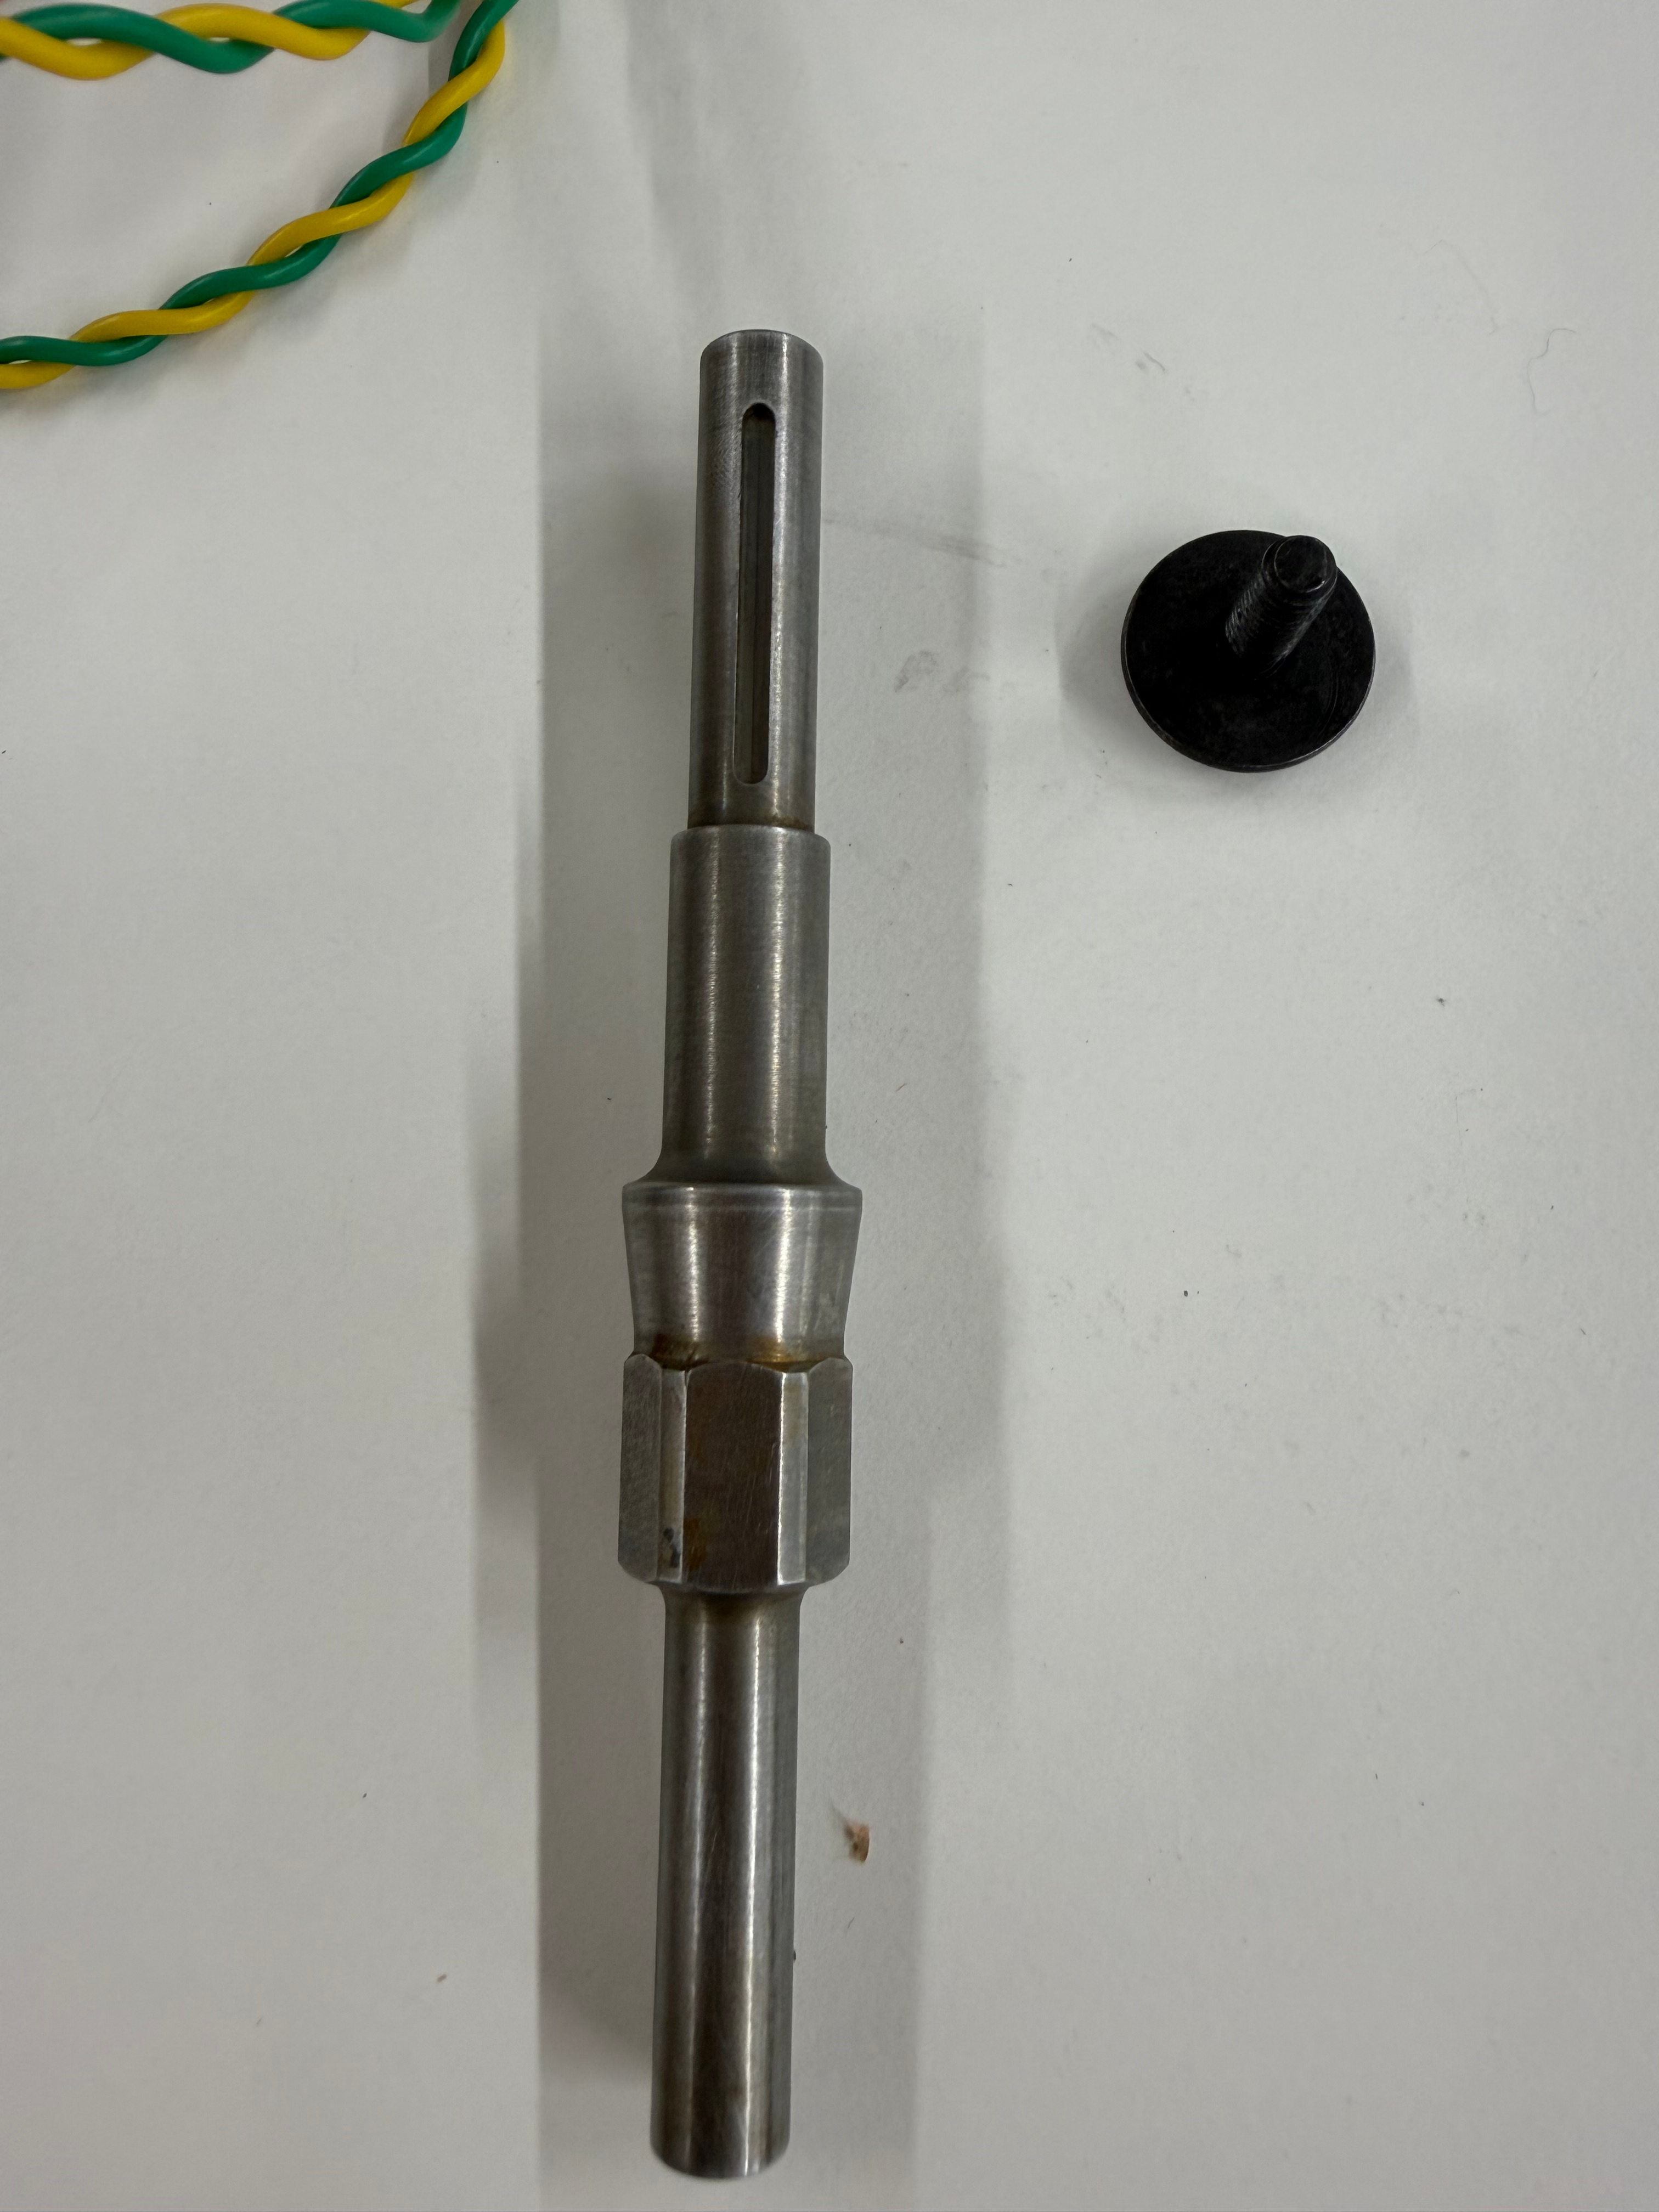
\includegraphics[width=0.31\textwidth]{media/image5.png}
\hfill
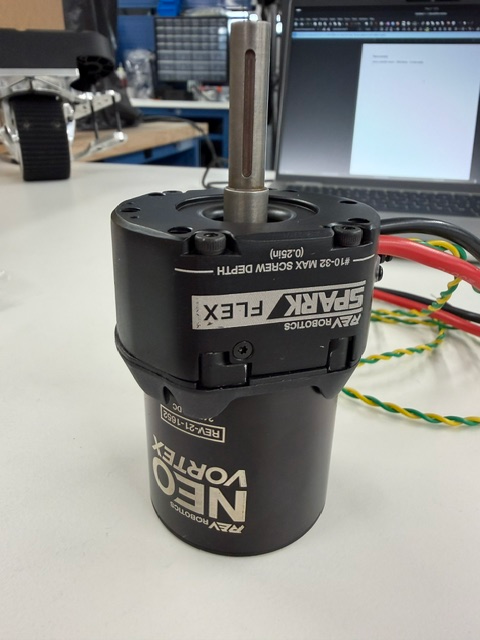
\includegraphics[width=0.31\textwidth]{media/image6.png}
\hfill
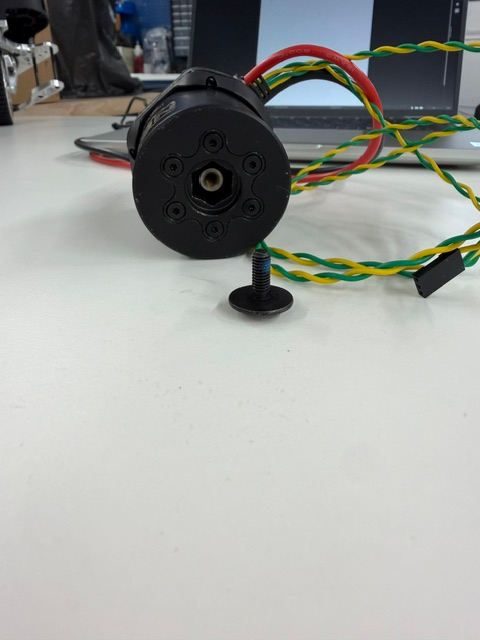
\includegraphics[width=0.31\textwidth]{media/image7.png}
\caption{Inserting the output shaft groove-up and securing it from the
opposite side of the motor.}
\end{figure}

\assemblystep{Assemble Remaining Motors}
Repeat the Motor Assembly steps seven more times to have 8 motors total.